\documentclass{beamer}
\usepackage{latexsym}
\usepackage{amssymb}
\usepackage{amsbsy}
\usepackage{alltt}
\usepackage{tikz}
\usepackage{stmaryrd}

\newcommand{\imp}{\Rightarrow}
\newcommand{\etal}{\textit{et. al}}
\newcommand{\adhoc}{\textit{ad hoc}}
\newcommand{\ie}{\textit{i.e.}}
\newcommand{\etc}{\textit{etc}}
\newcommand{\eg}{\textit{e.g.}}
\newcommand{\konst}[1]{\ensuremath{\mbox{\bf{#1}}}}
\newcommand{\nil}{\konst{[\,]}}
\newcommand{\cons}[2]{{#1}\boldsymbol{:}\boldsymbol{:}{#2}}
\newcommand{\hollamb}{\boldsymbol{\lambda}}
\newcommand{\itelse}[3]{\mbox{$\mbox{\tt if}\ {#1}\ \mbox{\tt then}\ {#2}\
    \mbox{\tt else}\ {#3}$}}
\newcommand{\set}[1]{\{ {#1} \}}
\newcommand{\Lang}[1]{\ensuremath{{\cal L}({#1})}}
\newcommand{\inbox}[1] {\begin{center}
                         \framebox{\parbox{0.984\textwidth}{#1}}
                         \end{center}}
\newcommand{\den}[1]{%
  \ensuremath{%
    \left\llbracket{#1}
    \right\rrbracket}}

% for backslashes in alltt environments
\newcommand{\bs}{\texttt{\symbol{92}}}

\usetikzlibrary{shapes}


\begin{document}

\begin{frame}\frametitle{SPLAT is where it's at!}

\hspace{50mm}
{\small
\begin{tabular}{l}
Konrad Slind \\ Collins Aerospace \\ CASE Project PI visit \\ May 22 2019
\end{tabular}
}

\end{frame}

\begin{frame}\frametitle{Overview}

\konst{SPLAT}\footnote{SPLAT = \textit{Semantic Properties for Language and Automata Theory}} is a plugin to the Collins "Architecture-Level Designer
Workbench".

\vspace{10mm}

\konst{SPLAT} provides support for adding filters between components
in order to prevent reception of badly formed or malicious messages.

\end{frame}

\begin{frame}\frametitle{Functionality}

\begin{itemize}
  \item Input: an AADL architecture annotated with filter specifications
\vspace*{5mm}
  \item Output: a logical theory containing the
following elements for each filter specified in the architecture:

\begin{itemize}

  \item[-] declaration of the record and enumeration type(s) corresponding to 
    the filter input

  \item[-] definition(s) of the wellformedness of the filter input

  \item[-] a table-driven DFA that renders a pass-fail verdict on messages,
    allowing only wellformed messages to pass

  \item[-] encoder and decoder mapping between records and the message format

  \item[-] theorems showing the correctness of the DFA.

\end{itemize}
\end{itemize}
\end{frame}

\begin{frame}\frametitle{Picture}
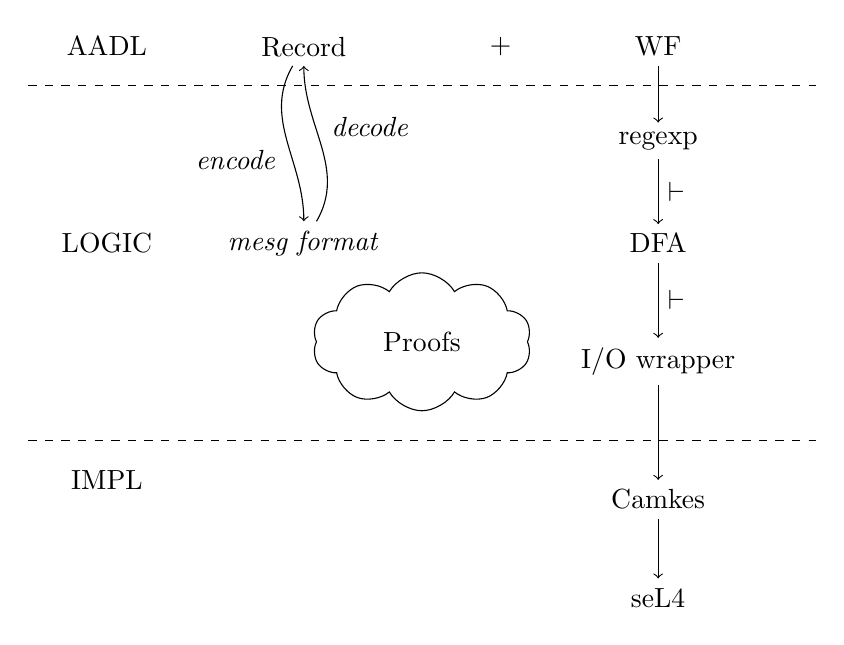
\begin{tikzpicture}[auto]
\node (AADL) at (1,0) {AADL};
\node (RECD) at (3.5,0) {Record};
\node () at (6,0) {+};
\node (WF) at (8,0) {WF};
\node (LOGIC) at (1,-2.5) {LOGIC};
\node (MESG) at (3.5,-2.5) {\textit{mesg format}};
\node (REGEXP) at (8,-1.2) {regexp};
\node (DFA) at (8,-2.5) {DFA};
\node (IOWRAP) at (8,-4) {I/O wrapper};
\node (CLOUD) [cloud, draw,cloud puffs=10,cloud puff arc=120, aspect=2, inner ysep=1em] at (5,-3.75) {Proofs};
\node (IMPL) at (1,-5.5) {IMPL};
\node (CAMKES) at (8,-5.75) {Camkes};
\node (SEL4) at (8,-7) {seL4};
\draw [dashed] (0,-0.5) -- (10,-0.5);
\draw [dashed] (0,-5) -- (10,-5);
\draw [->] (WF) to (REGEXP);
\draw [->] (REGEXP) to node{$\vdash$} (DFA);
\draw [->] (DFA) to node{$\vdash$} (IOWRAP);
\draw [->] (IOWRAP) to (CAMKES);
\draw [->] (CAMKES) to (SEL4);
\draw [->] (RECD) to [out=-120,in=north] node[swap]{\textit{encode}}(MESG);
\draw [->] (MESG) to [out=60,in=south] node[swap]{\textit{decode}}(RECD);
\end{tikzpicture}

\end{frame}

\begin{frame}\frametitle{What kinds of records are handled?}

  A field can have:

\begin{itemize}
 \item signed/unsigned numbers
 \item number constants
 \item elements of enumerated types
 \item character and string literals
 \item arrays
 \item sub-records (records of records ...)
\end{itemize}

\vspace*{5mm}

Not handled (yet): 

\begin{itemize}
 \item floating point numbers
 \item recursive types (lists, trees, etc)
\end{itemize}

\end{frame}

\begin{frame}\frametitle{Wellformedness}

Expressed as constraints on fields

\vspace*{5mm}

\begin{itemize}
 \item numeric fields can be given interval constraints
 \item constant fields can directly specified
 \item enumeration fields can be restricted to only a subset of the enumeration
\end{itemize}

\vspace*{5mm}

Basis of our approach is that interval constraints on numbers can be expressed by regexps.

\vspace*{5mm}
\noindent\textbf{NB}
Inter-field constraints not allowed (e.g. \textit{field X is the
  length of field Y} cannot work in \konst{SPLAT})

\end{frame}


\begin{frame}[fragile]\frametitle{Example}

Record type declaration

\begin{verbatim}
  gps = <| lat : int ;
           lon : int ;
           alt : int |>
\end{verbatim}

Wellformedness

\begin{verbatim}
  good_gps recd <=>
      -90 <= recd.lat /\ recd.lat <= 90 /\
      -180 <= recd.lon /\ recd.lon <= 180 /\
      0 <= recd.alt /\ recd.alt <= 17999
\end{verbatim}

\end{frame}


\begin{frame}\frametitle{Message format}

Wellformedness is a high level predicate, it applies at the level of
record datatypes. The message format, however, is what actually gets
sent in a communication.

\vspace*{5mm}

The following dimensions need to be addressed in order to truly pin
down the message format:

\begin{itemize}
 \item representation: twos complement, sign-magnitude, funky encodings
 \item Signed/unsigned numbers
 \item Field width
 \item Byte order (also bit order)
 \item Order of layout of fields
 \item Skipped fields
 \item Padding, markers, magic numbers, etc
 \item Packing
 \item ... and probably more
\end{itemize}

\end{frame}


\begin{frame}[allowframebreaks,fragile]\frametitle{Example (contd)}

\begin{itemize}

\item Pick an encoding of ints (sign-magnitude), with encoder/decoder
  \konst{encZ}/\konst{decZ}. 

\item Encoder (autogenerated)

\begin{verbatim}
  encode(gps) = 
    CONCAT [encZ 1 gps.lat; 
            encZ 1 gps.lon; 
            encZ 2 gps.alt]
\end{verbatim}

\item Decoder (autogenerated)

\begin{verbatim}
  decode s =
    case s
     of [a;b;c;d;e;f;g] =>
        SOME <| lat := decZ [a;b];
                lon := decZ [c;d];
                alt := decZ [e;f;g] |>
      | otherwise => NONE
\end{verbatim}

\framebreak

\item A regexp is autogenerated from the constraints. Each field
  is described by an \emph{interval regexp} for that field.

\vspace*{5mm}

\item Regexp (concrete syntax)

\begin{verbatim}
  \i{~90,90}\i{~180,180}\i{0,17999}
\end{verbatim}

\vspace*{5mm}

\item Regexp (AST, prettyprinted)

\begin{verbatim}
  ([+][\000-Z] | [-][\001-Z])
  ([+][\000-\180] | [-][\001-\180])
  ([+] ([\000-O][F] | .[\000] | .[\001-E]))
\end{verbatim}

\framebreak

\item Regexp (AST, raw)

{\tiny
\begin{verbatim}
Cat
 (Or [Cat (Chset (Charset 8796093022208w 0w 0w 0w))
      (Chset (Charset 18446744073709551615w 134217727w 0w 0w));
      Cat (Chset (Charset 35184372088832w 0w 0w 0w))
          (Chset (Charset 18446744073709551614w 134217727w 0w 0w))])
(Cat
 (Or [Cat (Chset (Charset 8796093022208w 0w 0w 0w))
          (Chset (Charset 18446744073709551615w 
             18446744073709551615w 9007199254740991w 0w));
      Cat (Chset (Charset 35184372088832w 0w 0w 0w))
          (Chset (Charset 18446744073709551614w 
            18446744073709551615w 9007199254740991w 0w))])
(Cat (Chset (Charset 8796093022208w 0w 0w 0w))
     (Or [Cat (Chset (Charset 18446744073709551615w 65535w 0w 0w))
              (Chset (Charset 0w 64w 0w 0w));
          Cat (Chset (Charset 18446744073709551615w 
                18446744073709551615w 18446744073709551615w 
                18446744073709551615w))
              (Chset (Charset 1w 0w 0w 0w));
          Cat (Chset (Charset 18446744073709551615w 
                18446744073709551615w 18446744073709551615w 
                18446744073709551615w))
              (Chset (Charset 18446744073709551614w 63w 0w 0w))])))
\end{verbatim}
}

\end{itemize}
\end{frame}

\begin{frame}[allowframebreaks]\frametitle{Formal properties}

A collection of relationships need to hold between the regexp, the
wellformedness condition, the encoder and the decoder:

\vspace*{5mm}

\begin{itemize}

\item \textit{The record is wellformed iff its corresponding message passes the filter}.
Formally:

\[ \forall g : \mathit{gps}.\ \konst{good\_gps}(g) 
  \iff \konst{encode}(g) \in \Lang{\mathit{regexp}}
\]

\begin{itemize}

\item[-]  This connects the filter behavior to the high-level property
$\konst{good\_gps}(g)$ used in compositional reasoning with AGREE.
  
\vspace*{3mm}

\item[-] L-to-R reading (sender side): if the record is wellformed the
  corresponding message will be accepted.

\vspace*{3mm}

\item[-] R-to-L reading tells us that \konst{encode} is ``good'' 

\end{itemize}

\framebreak

\item \textit{If a message passes the filter then it will decode into a wellformed record}.
Formally:

\[ \forall s.\; s \in \Lang{\mathit{regexp}}
   \imp \konst{good\_gps}(\konst{valOf}(\konst{decode}(s))) 
\]

\begin{itemize}

\item[-] This is a \emph{receiver-side} property

\vspace*{3mm}
  
\item[-] The checking of the message for wellformedness is
  accomplished by the filter, before the decoder gets called.

\vspace*{3mm}

\item[-] Maybe be possible to strengthen this to an iff, but not sure it's useful.

\end{itemize}

\framebreak

\item \textit{decode of encode is the identity}. Formally:

\[ \forall g.\; \konst{decode}(\konst{encode}(g)) = \konst{SOME}(g) \]

We attempt to prove this property, although it is not always true
(e.g. when some fields are superfluous to a message and the encoder
 omits them).

\item \textit{encode is an injection (1-1 function)}. In other words, encoding
  doesn't map two different records to each other.  We don't (yet) try
  to prove this property. It has the same issues as the round-trip
  property: dropping superfluous fields can result in identical messages.

\end{itemize}

\end{frame}

\begin{frame}\frametitle{Encode and decode}
  
Note that \konst{encode} and \konst{decode} are present in order to
express the desired properties, especially the first one. So they can
be regarded as artifacts primarily used to state correctness.

\vspace*{10mm}

We could also generate implementations, e.g. in CakeML, for
\konst{encode}/\konst{decode}.  It would be nice to generate versions
in popular languages for embedded systems.

\vspace*{10mm}

We could use the logic versions of \konst{encode}/\konst{decode} as
specifications against which to prove correctness of implementations
of \konst{encode}/\konst{decode} by others in standard PLs.

\end{frame}

\begin{frame}[allowframebreaks] \frametitle{Discussion}

\begin{itemize}

\item \konst{SPLAT} deliberately takes a formal language approach, in which
we try to apply formal language technology (e.g. regexps, grammars,
DFAs and DPDAs).

\vspace*{5mm}

\item This has benefits and limitations. The main limitation is that
  the functionality of some (many?) filters cannot be captured by a
  regular expression or with a grammar.

\vspace*{5mm}

\item A common question is \textit{``Why bother? Can't you just write (or generate) the
relatively simple validity checkers and verify them?''}

\framebreak

Response:
 
\begin{itemize}

\item[-] \konst{SPLAT} filters run exclusively at the bitstring level. There is
  no interpretation of data. Seems that this should lead to fast and
  inherently uniform execution.

\vspace*{3mm}

\item[-] The validity checker approach requires (essentially) parsing
  messages into records and then running the validity checks. 

\vspace*{3mm}

\item[-] For complex messages the validity checker may itself be complex.

\vspace*{3mm}

\item[-] For long messages, the input need not be stored in
  memory. State machines go character-by-character, so they need very
  little space (other than to store their static tables, which may be large).

\end{itemize}
\end{itemize}

\end{frame}

\begin{frame}\frametitle{Future work}

\begin{itemize}

\item Ongoing discussion with colleagues on adopting (or creating)
  an intermediate language for expressing message formats

\vspace*{2mm}

\item Performance and scaling

\vspace*{2mm}

\item Extend \konst{SPLAT} to CFLs and produce filters for complex tree-shaped data

\vspace*{2mm}

\item Extend to handle features not supported by formal language
  technology (e.g. length fields)

\end{itemize}

\end{frame}


\end{document}
